% +---------------------------------------------------------------+
% | Author :    Noémie Plancherel, HEIG-VD
% | Date :      16.10.2022
% +---------------------------------------------------------------+

\chapter{LastPass}
\label{ch:lastpass}

Ce chapitre sera dédié à l'analyse sécuritaire de l'application LastPass. Nous allons utiliser l'extension de navigateur sur Google Chrome. Il existe également des applications desktop, cependant les versions ne sont pas proposées sur le site officiel car ils mettent en avant uniquement l'extension de navigateur. Nous n'allons donc pas nous concentrer sur l'application desktop et uniquement analyser l'extension de navigateur. 

\section{Environnement}

\begin{table}[H]
	\centering
	\begin{tabular}{ll}
		\hline
		Logiciel           & Version        \\ \hline
		Windows 11         & 10.0.22621     \\
		Google Chrome      & 106.0.5249.119 \\
		LastPass Extension & 4.102.1        \\ \hline
	\end{tabular}
\caption{Environnement utilisé pour LastPass}
\end{table}

\section{Critères d'analyse}

Comme précisé précédemment, nous allons dans un premier temps définir tous les critères que nous souhaitons analyser
afin d'évaluer la sécurité du gestionnaire LastPass. Ainsi, nous avons établi les critères suivants:

\begin{itemize}
	\item Master password
	\item Choix cryptographiques
	\begin{itemize}
		\item Chiffrement
		\item Dérivation des clés
		\item Authentification
	\end{itemize}
	\item Fonctionnalités proposées
	\begin{itemize}
		\item Génération de mots de passe
		\item Auto-complétion de champs
		\item Presse-papier
	\end{itemize}
	\item Stockage
	\item Mémoire
\end{itemize}

Pour chaque critère, nous analyserons sa sécurité et nous l'évaluerons afin d'indiquer s'il s'agit d'une fonctionnalité sûre ou d'une faiblesse qui aurait besoin d'être corrigé avec une contre-mesure.

Nous allons également citer quelconque faiblesse ou faille identifiée et connue pour chaque critère afin de se concentrer sur certains points lors de notre analyse et de constater si la faiblesse existe encore ou pas.

\section{Master password}
Lors de l'inscription de l'utilisateur, LastPass va demander d'entrer un master password afin de pouvoir créer le coffre-fort. Étant donné que LastPass dérive la clé de chiffrement à l'aide du username et du master password, il est important que ce dernier soit fort et aléatoire afin d'éviter des attaques par dictionnaire. 

LastPass à ajouter les critères suivants afin de valider le master password entré par l'utilisateur:
\begin{itemize}
	\item minimum de 12 caractères
	\item minimum de 1 chiffre
	\item minimum de 1 majuscule
	\item minimum de 1 minuscule
	\item pas l'adresse e-mail utilisée pour le username
\end{itemize}

Afin d'estimer la force du master password pour contrer une attaque de brute force, nous pouvons calculer la complexité d'un mot de passe avec les critères minimum pour réaliser s'ils sont suffisants. On sait que pour les 12 caractères exactement il y a 3 possibilités différentes qui sont des caractères alphanumériques sensibles à la casse. Donc 26 lettres minuscules, 26 lettres majuscules et 10 chiffres. Ainsi, nous pouvons déduire:

\begin{center}
$n = 26 + 26 + 10$ \\
$c = n^{12}$ \\
$c = 3.226266762 \times 10^{21}$ \\
\end{center}

Nous constatons que le nombre de combinaisons est grand et que les critères semblent assez suffisant afin d'éviter des attaques. 

En se basant sur l'étude de Hives Systems\cite{hives}, avec une GPU récente et puissante (RTX 3090), il faudrait 200 ans à un attaquant pour brute force le master password. Ce qui est pour l'instant un nombre de temps acceptable mais il serait nécessaire d'y faire attention pour les mois à venir.

De plus, LastPass utilise l'algorithme PBKDF2-SHA2 avec 100'100 rounds pour dériver le master password et le stocker sur la base de données utilisateurs sur leurs serveurs. Ce dernier est premièrement dérivé avec l'adresse e-mail comme salt, puis une deuxième fois afin de créer un hash d'authentification. Il est stocké dans la base de données en utilisant un salt aléatoire (un différent par utilisateur) et en le hashant de nouveau avec PBKDF2-SHA2 100'100 rounds et Scrypt.

Ainsi, cela amène une couche sécuritaire non-négligeable qui protège un maximum le master password de l'utilisateur. 

\subsection{Entropie}
Nous pouvons calculer l'entropie du master password minimum exigé par LastPass:

\begin{center}
	$E = log_2(62^{12})$ \\
	$E = 71.4503$
\end{center}

D'après l'échelle que nous avons proposé dans la section \ref{entropie}, les mots de passe générés sont raisonnables, c'est-à-dire qu'ils sont acceptables, mais il serait nécessaire d'accompagner les master password d'une bonne implémentation de l'authentification de l'utilisateur.

\subsection{Brute-force authentification}

L'étude de 2020 de l'université de York\cite{carr}, liste une faiblesse découverte lors de son analyse sur plusieurs gestionnaires de mots de passe, notammant LastPass. Il indique que LastPass a une partielle contre-mesure contre le brute-force sur les extensions de navigateur. Nous avons testé d'entrer plusieurs master passwords faux, dans un premier temps dans un mode en ligne et dans un second temps en mode hors-ligne.

\textbf{En ligne}

Lors d'environ 6 essais de master password faux, l'authentification est bloquée pendant 5 minutes et un e-mail est envoyé à l'utilisateur. Cette contre-mesure est efficace à contrer les attaques brute-force, comme les attaques par dictionnaire. Pour un attaquant, cela ferait à peu près 72 essais par heure, ce qui prendrait énormément de temps pour brute-forcer. Ainsi, ces mesures ralentissent considérablement les attaques et peut les prévenir. 

\textbf{Hors-ligne}

Lors de brute-force hors-ligne, il n'y aucun nombre d'essais maximum. Ainsi, aucune protection n'a été ajoutée afin de contrer des attaques. Il serait nécessaire d'ajouter des contre-mesures afin d'éviter toute faille car pour une telle attaque, l'attaquant n'a pas besoin de privilèges ni de l'interaction de l'utilisateur. Néanmoins, l'attaque s'appuie, entre autres, sur la complexité du mot de passe. Ainsi, nous remarquons que la politique du master password proposée par LastPass permet de configurer des mots de passe fort, ce qui pourrait permettre de ralentir considérablement des attaques de brute-force.

\section{Choix cryptographiques}
\subsection{Chiffrement}
Pour le chiffrement de toutes les données du gestionnaire de mots de passe, LastPass utilise AES-CBC 256. Cet algorithme est communément utilisé et est encore recommandé en 2022\cite{ecrypt}, cependant il est important d'utiliser un IV aléatoire et unique pour chaque élément chiffré afin d'éviter la réutilisation d'IV. 
\subsection{Dérivation des clés}
Comme cité précédemment, pour la dérivation des clés afin de créer la clé de chiffrement et le hash d'authentification, LastPass utilise PBKDF2-SHA256 avec des rounds de 100'100 et 100'101 (par défaut, augmentable dans les paramètres de l'application). En se référant à Ecrypt, ils suggèrent un minimum de 40'000 rounds, donc suffisamment de rounds sont effectués sur LastPass. Le salt utilisé pour la dérivation du master password est le username, donc l'adresse e-mail de l'utilisateur. Pour bien, il serait mieux d'utiliser un salt généré aléatoirement avec un PRNG afin de s'assurer qu'il soit aléatoire et unique. Néanmoins, LastPass s'assure correctement que l'adresse e-mail est unique et n'est pas encore utilisée par un autre utilisateur, ainsi ils garantissent qu'aucune clé de chiffrement ne pourra être identique.

En 2022, il est recommandé d'utiliser Argon2 à la place de PBKDF2 pour les nouveaux systèmes car ce dernier n'est pas résistant à certaines attaques (GPU par exemple).\cite{medium}

Ainsi, il serait intéressant pour LastPass d'ajouter Argon2 comme algorithme supporté pour la création des clés.
\subsection{Authentification}
Pour authentifier un utilisateur, LastPass va générer un hash d'authentification en dérivant deux fois le master password avec PBKDF2-SHA2. Ce dernier sera par la suite stocké dans la base de données de l'utilisateur en l'hashant une fois de plus avec PBKDF2-SHA2 avec un salt aléatoire (généré par utilisateur). En plus, LastPass le hashe une fois de plus avec l'algorithme Scrypt, qui ajoute une protection supplémentaire aux attaques par dictionnaire et au brute force. Ces deux dernières manipulations sont effectuées du côté serveur.
\section{Fonctionnalités proposées}
Dans les sections suivantes, nous allons évaluer la sécurité dans quelques fonctionnalités proposées par LastPass. 
\subsection{Génération des mots de passe}
\label{lp_pw}
LastPass offre la fonctionnalité de générer des mots de passe automatiquement lors de l'ajout d'une entrée mot de passe dans le gestionnaire. Il est important d'évaluer la force des mots de passe générés afin de s'assurer que leur sécurité est garantie.

LastPass propose la génération suivante:

\begin{table}[H]
	\centering
	\begin{tabular}{llll}
		\hline
		 Longueur supportée & Composition par défaut      & Taille par défaut & Symboles proposés              \\ \hline
		 1-99               & {[}A-Za-z0-9{]} & 12                & *!\#\$\&\%@\textasciicircum{} \\ \hline
	\end{tabular}
\caption{Fonctionnalités de LastPass pour la génération de mots de passe}
\end{table}

Une option que LastPass ne demande pas par défaut lors de la génération d'un mot de passe est d'ajouter au minimum un caractère par set de caractères\footnote{Nous définissons un set de caractères par [A-Z] par exemple} mis à disposition. Ce qui pourrait faire baisser le taux d'aléatoire et générer des mots de passe moins forts. 

Au niveau des des symboles proposés pour la génération, nous remarquons qu'il n'y a pas une grande variation de caractères proposés, ce qui pourrait amener moins d'aléatoire lors de la génération de mots de passe.

De plus, sur l'extension, il y a la possibilité de générer des mots de passe "facile à dire" ou "facile à lire" pour aider l'utilisateur à la mémorisation. Cette fonctionnalité pourrait également baisser la sécurité dans la génération de mots de passe si la longueur n'est pas suffisante (minimum 12). 

Une étude réalisée en 2021\cite{oesch} sur l'évaluation de la qualité de la génération de mots de passe, a testé l'aléatoire et la robustesse de la génération. Cette dernière à pris en compte les différents sets de caractères et la longueur du mot de passe. Ainsi, nous allons nous baser sur cette étude en effectuant des tests sur la génération de mots de passe sur LastPass. Pour ce faire, nous allons générer le pool de données suivant:

\begin{itemize}
	\item lettres majuscules / minuscules (ll)
	\item lettres majuscules / minuscules + chiffres (lc)
	\item lettres majuscules / minuscules + symboles (ls)
	\item symboles + chiffres (sc)
	\item lettres majuscules / minuscules + symboles + symboles (all)
\end{itemize}

Pour chaque composition, nous allons générer 10'000 mots de passe aléatoires et avec à chaque fois 12, 16 et 20 caractères. 12 caractères étant la valeur par défaut sur LastPass, nous avons décidé de commencer à cette valeur-ci pour évaluer sa robustesse.

Afin de récupérer tous les mots de passe générés par l'extension, nous avons créé un fichier Java avec Selenium, qui permet de créer des scripts pour automatiser le navigateur. Le script se trouve à cet endroit dans le rapport \ref{script_gen_last}\footnote{Pour des raisons de place et de redondance, le script en entier n'a pas été ajouté, cependant pour chaque composition la logique est la même pour le code}. 

Pour évaluer la qualité de l'aléatoire et la robustesse, nous allons utiliser un outil créé par Daniel Wheeler\cite{197177} qui vérifie la popularité d'un mot de passe selon plusieurs sources - des sets de mots de passe fuités, des noms communs, le mots communs sur Wikipédia. Le programme va également regarder des motifs communs, comme par exemple des dates, des séquences répétées ou du clavier. En fonction de tous ces facteurs, il va estimer le nombre d'essais qu'un attaquant aura besoin afin de trouver le mot de passe de l'utilisateur. Le résultat du nombre d'essais est présenté en 4 catégories d'attaques sur mots de passe différentes qui permettent de visualiser tous les résultats possibles:

\begin{itemize}
	\item \textbf{Online Throttling} (100 essais/heure) est une attaque en ligne sur un service qui limite le nombre d'essais lors de l'authentification
	\item \textbf{Online No Throttling} (10/seconde) est une attaque en ligne où il n'y pas de nombre d'essais maximum ou que l'attaquant a réussi à le contourner
	\item \textbf{Offline Slow Hashing} ($1e^4$/seconde) est une attaque hors-ligne où les mots de passe ont des fonctions de hachage lentes (comme PBKDF2).
	\item \textbf{Offline Fast Hashing} ($1e^{10}$/seconde)	est une attaque hors-ligne où les mots de passe ont des fonctions de hachage rapides (comme M5, SHA1).
\end{itemize}

Ainsi, nous avons utilisé l'outil pour Java\footnote{\href{https://github.com/nulab/zxcvbn4j}{https://github.com/nulab/zxcvbn4j}} afin d'évaluer la robustesse de tous les mots de passe générés dans l'étape précédente. Le code s'inspire grandement de l'outil original\footnote{\href{https://github.com/dropbox/zxcvbn}{https://github.com/dropbox/zxcvbn}}, mais il y a quelques différences lors des estimations. Toutefois, nous avons choisi l'outil Java afin de pouvoir écrire un script qui teste tous les mots de passe générés.

Le script\ref{script_test_last} implémenté a pour but de récupérer les mots de passes les plus faiblement générés en fonction du résultat du nombre d'essais et du nombre de caractères. L'outil retourne le score du mot de passe en $log_{10}$ pour que les nombres ne soient pas trop élevés. Ainsi, l'étude propose cette échelle d'évaluation suivante en fonction du score du mot de passe:

\begin{enumerate}
	\item $< 3$ ($log_{10}$), mot de passe risqué et trop vite devinable
	\item $< 6$, très devinable et protégé contre les attaques en ligne throttled
	\item $< 8$, quelque peu devinable et protégé contre les attaques en ligne unthrottled
	\item $< 10$, suffisement non-devinable et modérément protégé contre les attaques hors-ligne avec des fonctions lentes
	\item $>= 10$, non-devinable et forte protection contre les attaques hors-ligne avec des fonctions lentes	
\end{enumerate}

Pour les résultats \ref{lp_result}, nous allons parler de quelques scores intéressants. Néanmoins, en général les résultats sont plutôt bons. Très occasionnellement, le générateur produit des mots de passes faibles (environ 1 fois sur 400), ce qui peut être tout à fait normal pour un générateur vraiment aléatoire. Néanmoins, d'après nos tests, le plus petit score se situe au niveau 4/5, ce qui est tout de même un bon score et un mot de passe plutôt fort et aléatoire. 

Pour les 3 longueurs de mots de passe différents, la composition où le nombre d'essais est le plus petit sont avec des symboles et des chiffres. Cette constatation est assez logique car son entropie est la plus basse de toute les compostions.

Au niveau des attaques, pour 12 caractères, nous constatons que les mots de passes sont assez vulnérables aux attaques hors-ligne, car le temps d'essais est assez court. Pour 16 caractères, pour les mots de passe les plus faibles, ils sont toujours un peu vulnérables aux attaques hors-ligne avec des fonctions de hachage rapides. Finalement, dès 20 caractères, nous constatons que tous les mots de passe sont fortement protégé contre tous les types d'attaques. 

\subsection{Auto-complétion}

Afin de se référer à des faiblesses déjà connues de LastPass, nous allons nous appuyer sur une étude de 2013\cite{youn} et une plus récente de 2020\cite{carr} qui documentent des vulnérabilités découvertes sur des extensions de navigateur de gestionnaires de mots de passe, où LastPass a également été analysé. Une vulnérabilité qui est ressortie dans les deux études, est le fait que LastPass ignore les sous-domaines lors de la comparaison des origines, ce qui viole la \textit{same-origin policy}. 

Ainsi, nous avons testé si la faille existe encore en enregistrant des identifiants pour le nom de domaine parent \verb|https://heig-vd.ch|:

\begin{figure}[H]
	\centering
	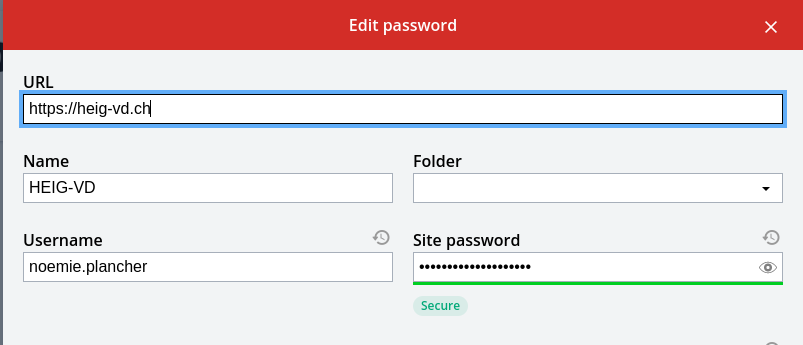
\includegraphics[width=15.5cm]{images/lp_heigvd.png}
	\caption{Identifiants pour heig-vd.ch enregistrés sur LastPass}
\end{figure}

\newpage

Ensuite, nous avons testé de nous connecter à un sous-domaine avec \\ \verb|https://webmail.heig-vd.ch|:
\begin{figure}[H]
	\centering
	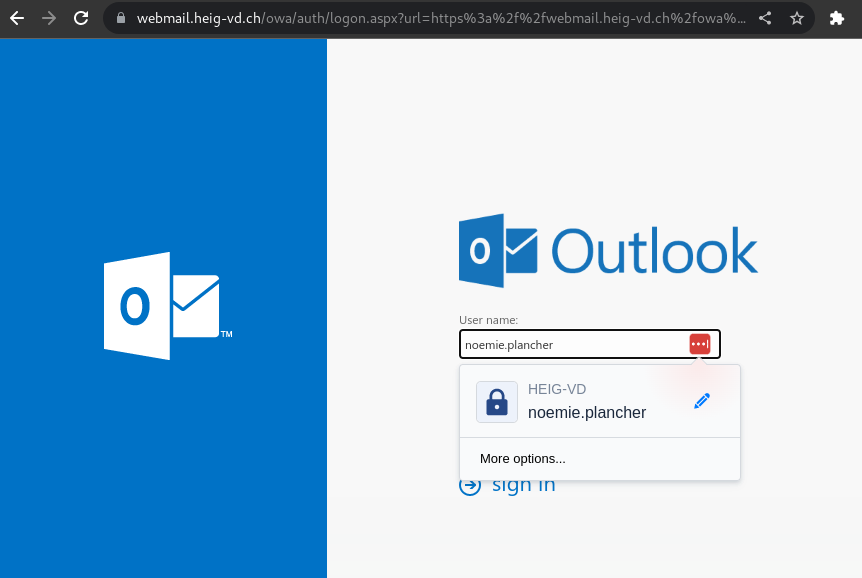
\includegraphics[width=15.5cm]{images/lp_webmail.png}
	\caption{Auto-complétion d'identifiants sur webmail.heig-vd.ch}
\end{figure}

Ainsi, nous constatons que LastPass propose les identifiants pour le sous-domaine car il les traite de la même manière.

Cette faiblesse pourrait être dangereuse car un attaquant pourrait potentiellement effectuer une attaque XSS en ajoutant un faux formulaire de connexion afin de récupérer les identifiants auto-complétés ou il pourrait utiliser l'HTML afin d'ajouter un formulaire de connexion sur le domaine client et ainsi voler des identifiants.

Néanmoins, sur LastPass, le résultat est aléatoire car la vulnérabilité n'apparaît pas pour chaque sous-domaine. En prenant notre exemple, avec le sous-domaine \verb|https://gaps.heig-vd.ch|, les identifiants ne sont pas proposés:

\begin{figure}[H]
	\centering
	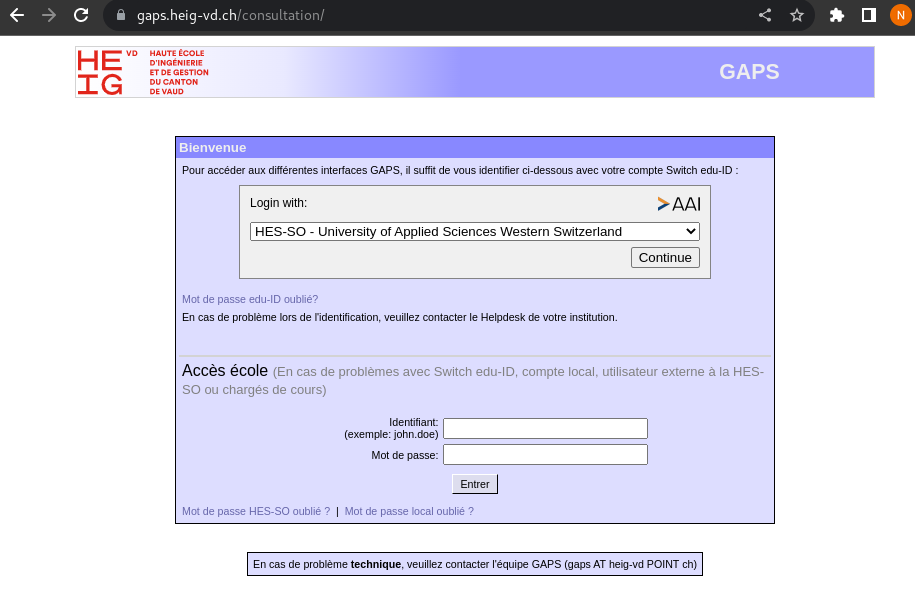
\includegraphics[width=15.5cm]{images/lp_gaps.png}
	\caption{Auto-complétion d'identifiants sur gaps.heig-vd.ch}
\end{figure}

Sinon, par défaut, LastPass auto-complète seulement les champs mais ne se connecte pas automatiquement (fonction modifiable dans les paramètres de l'entrée). Cela pourrait être critique car un attaquant pourrait effectuer une attaque XSS ou injection réseau et sans l'interaction de l'utilisateur, récupérer les identifiants qui ont été entrés dans le formulaire de connexion.

\subsection{Presse-papier}
La fonctionnalité de copier le mot de passe enregistré dans le presse-papier est souvent proposée lorsque le remplissage automatique de champs de connexion n'est pas proposée. Néanmoins, LastPass propose de copier le username, le mot de passe ou l'URL du site de connexion. 

Par défaut, LastPass nettoie le presse-papier après 60 secondes. Ce temps est correct au niveau sécurité cependant, pour une meilleure protection contre le sniffing de presse-papier, ce temps pourrait être réduit à 30 secondes maximum. L'utilisateur a également la possibilité de décocher cette case et que LastPass ne nettoie plus le presse-papier. Il est certain qu'il serait plus sécurisé d'enlever cette option afin d'éviter au maximum la perte ou le vol de données sensibles. 

Toutefois, il est compliqué de se protéger à 100\% de malwares de ce genre car à moins de ne pas permettre à l'utilisateur de copier ses mots de passe et d'effacer le presse-papier après un court instant, aucune protection n'est possible. Pour ce point, on ne peut que prévenir un maximum les utilisateurs qu'en leur exposant les risques et en leur demandant, par exemple, de verrouiller leur machine dès le moment où ils ne l'utilisent plus pour éviter qu'un attaquant sniffe leur presse-papier.
\section{Stockage}
LastPass fonctionne en ligne et hors-ligne\cite{9657969}, ainsi, il stocke des informations en local sur le disque de l'utilisateur afin d'avoir accès au coffre-fort et à toutes les données lorsque l'utilisateur n'est pas connecté à Internet. Tout dépend de l'OS et du navigateur, mais sur Windows 11 et Chrome, nous pouvons trouver une base de données SQLite à cet endroit: \\ \path{%AppData%\Local\Google\Chrome\UserData\Default\databases\chrome-extension_} 
	\\
	\path{hdokiejnpimakedhajhdlcegplioahd_0}. Nous pouvons trouver plusieurs tables différentes, dont \textit{LastPassData} où se trouvent les différentes entrées chiffrées du coffre-fort et le hash pour vérifier l'authenticité de la clé. 
	
	En se basant sur une démonstration d'attaque qui date de 2019\cite{p59}, il explique comment la fonction \textit{Remember Password} amène une vulnérabilité importante dans l'extension LastPass. Si la fonction de se rappeler le mot de passe et le mode hors-ligne sont activés, l'attaque peut réussir à récupérer le master password et le déchiffrer. Comme cité précédemment, une base de données est stockée en local chez l'utilisateur, ainsi c'est la table \textit{LastPassSavedLogins2} qui nous intéresse. Elle contient les champs suivants: username, password, last\_login, protected. En analysant le code Javascript \verb|server.js|, qui se trouve dans le fichier \verb|background.html| de l'extension, il est possible de voir comment est déchiffré le master password et ainsi écrire un script pour récupérer ce dernier en clair.
	
	Toutefois, cette attaque n'a pas pu être effectuée sur la version actuelle de l'extension car plus aucune information n'est stockée dans la table \textit{LastPassSavedLogins2}, malgré toutes les conditions remplies.
	
	\begin{figure}[H]
		\centering
		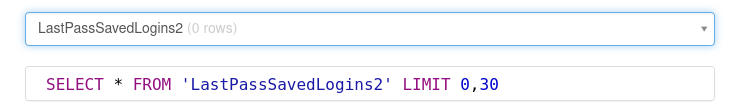
\includegraphics[width=15.5cm]{images/sql_lp.png}
		\caption{Table \textit{LastPassSavedLogins2} vide}
	\end{figure} 
	
	Nous avons analysé en profondeur le code disponible de l'extension et nous n'avons pas trouver de quelconque faiblesse qui nous permettrait de récupérer le master password enregistré. Les données qui transitent en local ont l'air d'être protégées en binaire, sans doute afin d'ajouter une couche de sécurité supplémentaire.
	
	Dès le moment où le master password n'est pas facilement récupérable et mis directement disponible pour les attaquants, cela permet de ralentir les personnes malveillantes et il est ainsi moins problématique d'avoir des données chiffrées en local.
\section{Mémoire}
D'après le whitepaper de LastPass, ils utilisent les \textit{Windows Crypto APIs}, misent à disposition par Windows, afin d'ajouter une couche supplémentaire de sécurité sur les appareils Windows. Ainsi, un test a été fait pour vérifier que le master password ou des informations sensibles, comme des mots de passe avec lesquels l'utilisateur aurait interagit, ne soient pas laissé en mémoire RAM lorsque le gestionnaire de mot de passe est verrouillé. 

Ainsi, nous avons effectué un dump de la mémoire du processus sur le disque et dû au fait que la mémoire est partiellement gérée par Windows avec ses APIs cryptographiques, il y a beaucoup de données qui sont chiffrées et illisibles. Néanmoins, avec un peu de recherche à l'aide de mes usernames que je connais, nous avons pu trouver tous les mots de passe du coffre-fort en clair dans la mémoire du processus. Nous pouvons le constater ci-dessous avec une entrée pour tumblr en recherchant le string "passworddec" sur le dump:
 
\begin{figure}[H]
	\centering
	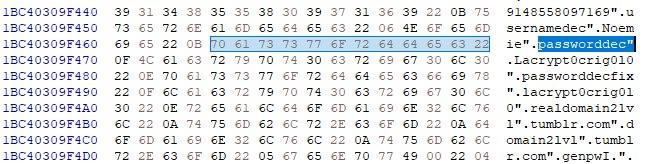
\includegraphics[width=15.5cm]{images/lp_pass.jpg}
	\caption{Entrée du coffre-fort LastPass en clair}
\end{figure} 

Cela veut donc signifier que LastPass charge tout le coffre-fort en mémoire dès que l'utilisateur se connecte et dès qu'elle est verrouillée, aucun nettoyage de la mémoire du processus n'est effectué. Toutefois, dès que le processus de l'application est stoppé, aucune donnée n'est visible en RAM.

\par\noindent\rule{\textwidth}{0.4pt}

Nous avons également effectué un autre test qui se base sur plusieurs attaques effectuées sur LastPass d'une étude de 2013\cite{zhao} et sur le travail de Bachelor de Léo Corthès\cite{leo}\footnote{Le travail étant confidentiel, il n'est pas possible de le visualiser, toutefois l'attaque expliquée s'appuie sur une étude de 2019\cite{p59}}. L'étude explique que l'extension utilise du javascript pour toutes les fonctionnalités, en incluant les opérations cryptographiques. Ainsi, la master key, qui est dérivée du master password et qui permet de chiffrer tout le coffre-fort, peut facilement se trouver dans le javscript sous le nom de variable  \verb|g_local_key|. Étant donné qu'on analyse une extension de navigateur, il est très commun d'avoir un fichier \verb|background.html| qui permet d'invoquer tous les scripts qui tournent en arrière-plan. De ce fait, en utilisant les outils de développeur sur Chrome, nous avons pu debuguer l'extension et chercher la master key pour afficher sa valeur. 

Nous avons décidé d'effectuer ce test\footnote{Les informations qui vont suivre ne seront pas censurées car il s'agit de valeurs d'exemples et non des valeurs réelles} lorsque le gestionnaire était verrouillé afin de simuler correctement une attaque possible. 

Premièrement, comme décrit dans le paragraphe plus haut, nous avons récupéré la valeur de \verb|g_local_key|, qui représente la master key, à l'aide des outils de développeur de Chrome.

\begin{figure}[H]
	\centering
	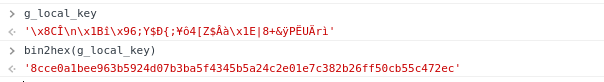
\includegraphics[width=10cm]{images/lp_master_key.png}
	\caption{Master key en mémoire}
\end{figure} 

Étant donné, que nous connaissons la valeur du master password (car il s'agit de mon compte) et que nous savons exactement comment LastPass dérive le master password (voir \ref{lp}), nous pouvons tester si la clé est réellement la master key :

\begin{lstlisting}[language=python, caption=Calcul de la master key sur LastPass]
>>> masterkey = hashlib.pbkdf2_hmac('sha256', b'Followthewhiterabbit98', b'noemie.plancherel@gmail.com', 100100, 32)
>>> binascii.hexlify(masterkey)

b'8cce0a1bee963b5924d07b3ba5f4345b5a24c2e01e7c382b26ff50cb55c472ec'

\end{lstlisting}

Ainsi, nous constatons que les deux clés sont similaires, c'est-à-dire que la variable \verb|g_local_key| est réellement la master key.

Avec cette information, nous pouvons à présent déchiffrer tout le coffre-fort. Comme précisé dans la section précédente, une base de données stocke tout le coffre-fort sur le disque de l'utilisateur. Pour cette partie, nous nous intéresserons à la table \textit{LastPassData} et au champ \textit{accts}. 

\begin{figure}[H]
	\centering
	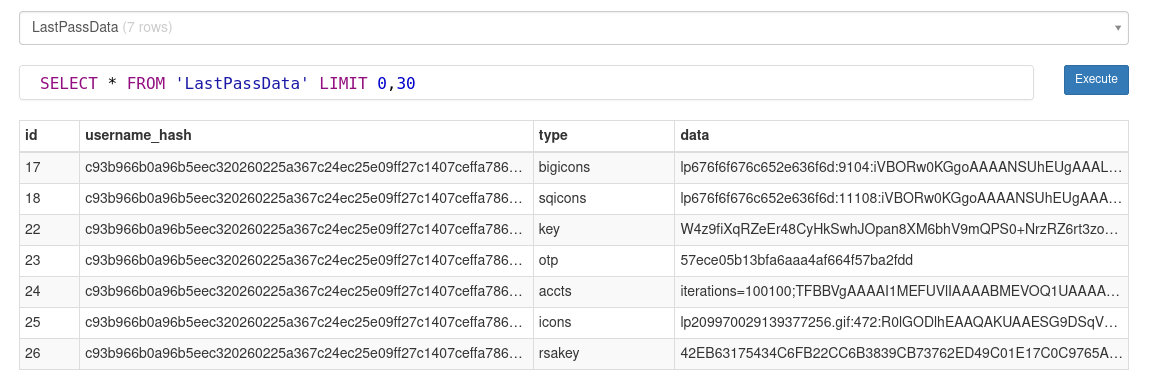
\includegraphics[width=15.5cm]{images/lp_data.png}
	\caption{Master key en mémoire}
\end{figure} 

Nous pouvons remarquer que le champ commence par le nombre d'itérations nécessaires pour dériver la master key et des données encodées en Base64 suivent. 

Les données en base64 représentent toutes les entrées du coffre-fort. L'étude de Derk Barten décrit la structure de chaque entrée qui possède des caractères de délimitations pour indiquer l'URL du site en clair, le username chiffré et le mot de passe chiffré.

Un script \ref{script_dec_lp} a été développé, inspiré par le celui proposé par Léo Corthès, afin de déchiffrer toutes les entrées du coffre-fort à l'aide de la master key récupérée à l'étape précédente. 

Toutefois, ce script a quelques limitations, il fonctionne uniquement pour les entrées basiques. LastPass propose plusieurs champs lors de l'enregistrement d'un mot de passe (username, mot de passe, URL, titre, notes ou encore un dossier). Ainsi, il est compliqué de savoir quelles entrées ont quels champs configurés et étant donné que toute la structure stockée est impactée, il n'est pas possible de déchiffrer exactement tous les champs de chaque entrée, néanmoins un maximum d'informations peuvent être récupérées sur le script, ce qui permet déjà à un attaquant d'avoir accès à quelques identifiants. 

Ces deux attaques de mémoire ont besoin de certaines conditions afin de pouvoir les exécuter sur les victimes.

\textbf{Attaque \#1 sur la mémoire du processus} 

\begin{itemize}
	\item Le gestionnaire de mot de passe doit être dans un état \textit{Locked} ou \textit{Unlocked}
\end{itemize}

\textbf{Attaque \#2 sur la mémoire du processus} 
\begin{itemize}
	\item Le gestionnaire de mot de passe doit être dans un état \textit{Unlocked}
	\item Le gestionnaire doit avoir le mode offline activé (par défaut il est activé)
	\item Le 2FA ou MFA ne doivent pas être configurés
\end{itemize}



\section{Récapitulatif de l'analyse}

Dans cette dernière section, nous allons établir un récapitulatif de toute l'analyse en passant par tous les points abordés, en ajoutant une évaluation de sécurité et en conseillant des contre-mesures nécessaires dans le cas où la faille est importante. 

% Please add the following required packages to your document preamble:
% \usepackage[table,xcdraw]{xcolor}
% If you use beamer only pass "xcolor=table" option, i.e. \documentclass[xcolor=table]{beamer}
\begin{landscape}
	\fontsize{8}{11}\selectfont
	\begin{longtable}[H]{llll}
		\cline{2-4}
		&
		\multicolumn{1}{c}{Critère analysé} &
		\multicolumn{1}{c}{Commentaire} &
		\multicolumn{1}{c}{Contre-mesures nécessaires ?} \\ \cline{2-4} 
		\cellcolor[HTML]{FFE135} &
		Master password &
		\begin{tabular}[c]{@{}l@{}}Les critères du master password sont forts,\\ cela permet de ralentir considérablement les\\ attaques de brute-force sur le master password, \\ cependant, l'entropie indique un mot de passe\\ moyen, ainsi il faudrait y faire attention pour les\\ mois à venir. Lorsque le gestionnaire est en mode \\ hors-ligne, il n'y a aucun nombre maximum \\ d'essais d'authentification, cela pourrait aider un \\ attaquant à effectuer du brute-force, néanmoins\\ étant donné que la politique des master password\\ de LastPass créée des mots de passe forts, l'attaque\\ prendrait du temps\end{tabular} &
		\begin{tabular}[c]{@{}l@{}}Il serait également bien d'ajouter un nombre d'essais \\ maximum de connexion, aussi lorsque le gestionnaire \\de mots de passe est hors-ligne, afin d'éviter au \\ maximum toute attaque de brute-force\end{tabular} \\ \hline
		\cellcolor[HTML]{228B22} &
		Chiffrement &
		\begin{tabular}[c]{@{}l@{}}L'algorithme utilisé pour le chiffrement du coffre-\\ fort est fort\end{tabular} &
		- \\ \hline 
		\cellcolor[HTML]{228B22} &
		Dérivation des clés &
		\begin{tabular}[c]{@{}l@{}}PBKDF2-SHA2 est efficace pour la dérivation \\ des clés. 100'100 rounds est également un nombre\\ assez grand pour permettre de ralentir au mieux \\ les attaques. Il serait bien d'ajouter un support pour\\ Argon2 afin de pouvoir proposer les deux\end{tabular} &
		- \\ \hline
		\cellcolor[HTML]{228B22} &
		Authentification &
		\begin{tabular}[c]{@{}l@{}}L'authentification auprès des serveurs est implémentée\\ de sorte à ce qu'il soit difficile de se faire passer par\\ l'utilisateur sans connaître son master password\end{tabular} &
		- \\ \hline
		\cellcolor[HTML]{228B22} &
		\begin{tabular}[c]{@{}l@{}}Génération de \\ mots de passe\end{tabular} &
		\begin{tabular}[c]{@{}l@{}}Les résultats sont plutôt bons; des mots de passes \\ faibles sont très occasionnellement générés et ils ont\\ de bons score au niveau du nombre d'essais pour les \\ deviner.\end{tabular} &
		\begin{tabular}[c]{@{}l@{}}Étant donné que par défaut, LastPass génère  des mots de passe \\ de 12 caractères, il serait bien de l'augmenter d'au moins 14 \\ caractères. De plus, il serait bien d'ajouter des symboles en plus de \\ ceux proposés afin de garantir un très bon aléatoire\end{tabular} \\ \hline
		\cellcolor[HTML]{FF9933} &
		Auto-complétion &
		\begin{tabular}[c]{@{}l@{}}Nous avons pu constater que des failles de 2013 sont\\ toujours présentes sur LastPass, notammant en ignorant\\ les sous-domaines lors de l'auto-complétion des champs.\\ L'option auto-remplissage des champs peut également\\ être dangereuse et être vulnérable à des attaques où un \\ attaquant ajouterait un formulaire de connexion caché.\end{tabular} &
		\begin{tabular}[c]{@{}l@{}}Une meilleure comparaison d'origine lors de l'auto-remplissage des \\ champs de formulaire serait nécessaire pour éviter toutes attaques. \\ De plus, l'option de auto-remplissage des champs étant activée \\ par défaut lors d'ajout d'une entrée dans le coffre-fort, il serait \\mieux de la désactiver et de laisser le choix à l'utilisateur ou d'avoir \\ une interaction avec ce dernier avant de remplir le champ pour \\qu'il puisse valider\end{tabular} \\ \hline
		\cellcolor[HTML]{228B22} &
		Presse-papier &
		\begin{tabular}[c]{@{}l@{}}Le timeout ajouté lors de la copie d'identifiants est correct.\\ Peut-être que baisser ce temps à 30-40 secondes serait\\ une meilleure solution, cependant il est compliqué de \\ se protéger à 100\% des attaques de sniffing, mais LastPass\\ ne peut rien faire de plus.\end{tabular} &
		- \\ \hline 
		\cellcolor[HTML]{FFE135} &
		Stockage &
		\begin{tabular}[c]{@{}l@{}}La base de données stockée local ne contient aucune \\ information en clair qui serait facile de récupérer directement.\\ La fonction de se rappeller du master password est sécurisée\\ car il n'y a pas la possibilité de récupérer le master password\\ directement dans une table de la base de données.\end{tabular} &
		\begin{tabular}[c]{@{}l@{}}En liaison avec les failles découvertes dans la  mémoire, il serait\\ nécessaire de désactiver le mode offline par défaut afin d'éviter \\ d'avoir des fichiers en local chez l'utilisateur. Cependant, sur \\LastPass afin de pouvoir désactiver ce mode, il faut avoir le 2FA \\ou MFA activé sur le gestionnaires. Ainsi, il faudrait également \\dissocier ces deux options.\end{tabular} \\ \hline
		\cellcolor[HTML]{CE2029} &
		Mémoire &
		\begin{tabular}[c]{@{}l@{}}Nous avons découvert deux failles assez critiques liées à la\\ mémoire et également au stockage de la base de données en \\ local. Premièrement, même quand le gestionnaire de mot de \\ passe est verrouillé, on a la possibilité de récupérer tous les\\ identifiants, avec mots de passe, en clair dans la mémoire du\\ processus car LastPass semble charger tout le coffre-fort en \\ mémoire et l'efface quand le processus est terminé. La seconde\\ faille permet de récupérer la master key depuis les outils de\\ développeurs de Chrome et de déchiffrer une grande partie du\\ coffre-fort grâce aux données stockées en local.\end{tabular} &
		\begin{tabular}[c]{@{}l@{}}La première faille est très critique, étant donné qu'un\\ attaquant pourrait effectuer un dump de la mémoire\\ assez facilement, même quand le gestionnaire de mots de\\ passe est verrouillé et il n'a pas besoin de privilèges\\ pour effectuer l'attaque. La sécurité à ajouter serait dans\\ un premier temps de s'assurer de nettoyer la mémoire\\ dès que le gestionnaire est verrouillé, puis s'assurer que\\ les données sensibles, tels que les mots de passe, soient\\ chiffrés dans la mémoire du processus, pour cela les OS\\ mettent à dispositon des APIs de cryptographie. De plus,\\ un timeout de session pour verrouiller le gestionnaire \\ après un certain temps serait une très bonne couche\\ sécuritaire en plus. Pour la seconde attaque, la première\\ contre-mesure à prendre serait de désactiver par défaut\\ le mode offline. Puis au niveau des outils de développeurs\\ de Chrome, il est assez difficile de gérer cette partie car\\ cela touche à tout l'arrière-plan de l'extension qui est \\ nécessaire quant à l'utilisation du gestionnaire.\end{tabular} \\ \hline
		\cellcolor[HTML]{FFE135} &
		Divers &
		\multicolumn{2}{l}{\begin{tabular}[c]{@{}l@{}}Nous pouvons ajouter un commentaire sur un élément que nous n'avons pas analysé mais qui est très important\\ à commenter; par défaut, l'extension ne se verrouille jamais, même quand le processus se termine. C'est à l'utilisateur \\ de se déconnecter manuellement. Cela pourrait être critique de ne jamais stopper la session, car un attaquant qui a accès \\au device déverrouillé de l'utilisateur, aura également accès au coffre-fort et à toutes les données en clair. Afin d'éviter \\ au maximum un vol de données, il serait recommandé d'ajouter un timeout de session par défaut (car actuellement il \\ est possible de le configurer dans les paramètres de LastPass).\end{tabular}} \\ \hline
		&
		&
		&
		\\
		\multicolumn{4}{l}{\textcolor{forestgreen(web)}{$\blacksquare$} Bonne sécurité, aucun contre-mesure à ajouter \textcolor{bananayellow}{$\blacksquare$} Sécurité moyenne, points à faire attention et quelques recommandations au niveau des contre-mesures} \\
		\multicolumn{4}{l}{\textcolor{deepsaffron}{$\blacksquare$} Sécurité faible, contre-mesures à prendre \textcolor{fireenginered}{$\blacksquare$} Sécurité très faible, contre-mesures à prendre rapidement car failles critiques} \\		      
	\end{longtable}
\end{landscape}